\documentclass[margin,line]{resume}
\usepackage{amsmath}

\usepackage[latin1]{inputenc}
\usepackage[english]{babel}
\usepackage[T1]{fontenc}
\usepackage{graphicx,wrapfig}
\usepackage{url}

\usepackage[colorlinks=true, a4paper=true, pdfstartview=FitV,
linkcolor=blue, citecolor=blue, urlcolor=blue]{hyperref}
\pdfcompresslevel=9


\setlength{\voffset}{-0.5in}
\setlength{\oddsidemargin}{-0.2in}
\setlength{\textwidth}{380pt}
% \setlength{\paperheight}{900pt}

\begin{document}

~
\vspace{-1cm}

{\sc \Large Curriculum Vitae ~~~~~~~~~~~~~~~~~~~~~~~~~~~~~~~~~~~~~~~~~~~~ \scriptsize update \today}
\begin{resume}
    % \vspace{0.5cm}
    
    % Picture:
%    \begin{wrapfigure}{R}{0.3\textwidth}
%        \vspace{-1cm}
%       \begin{center}
%       	\hspace{-0.5cm}
%       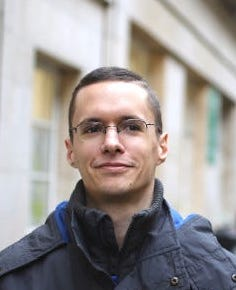
\includegraphics[width=0.25\textwidth]{ferraris_s}
%       \end{center}
%     \vspace{-1cm}
%    \end{wrapfigure}
    
    \section{\mysidestyle Contacts}
    
    Sebastiano Ferraris, PhD
    
    +44 775689xxxx
    
    \href{mailto:sebastiano.ferraris@gmail.com}{sebastiano.ferraris@gmail.com}

    $\triangleright$ \href{http://www.github.com/SebastianoF}{GitHub}\\
    $\triangleright$ \href{https://www.researchgate.net/profile/Sebastiano_Ferraris}{ResearchGate}\\
    $\triangleright$ \href{https://www.linkedin.com/in/ibis-redibis/}{LinkedIn}\\
    $\triangleright$ \href{https://scholar.google.com/citations?user=1tAeAI0AAAAJ&hl=en}{Google Scholar}\\
    $\triangleright$ \href{https://geospatial.netlify.app/posts/}{Blog}

%~

\section{\mysidestyle Studies \\ and \\ Works}


{\bf Data Scientist - \href{https://www.generalsystem.com/}{General System} - $2020$-Present} 
\vspace{0.1cm}
\begin{itemize}
    \item[] \hspace{-1.0cm} Geospatial data Science Services: Startup in stealth mode until April 2022
    \item[$\triangleright$] Developing prototypes to automate spatiotemporal data analysis at scale with clustering method, dashboards and \href{https://kepler.gl/}{KeplerGl} visualisation.
    \item[$\triangleright$] Collaborating with clients and domain experts to quickly and iteratively integrate feedback into prototypes.
    \item[$\triangleright$] Prototypes handover to production and DevSecOps teams.
    \item[$\triangleright$] Developing and \href{https://github.com/thegeneralsystem}{open sourcing} python libraries to provide users tooling and examples of the \href{https://assets.website-files.com/636ce900cf2e67aab6340642/643807134214aebc2b29849c_General%20System_The%20Data%20Flow%20Index%20Whitepaper%20_%20Nov%2022.pdf}{Data Flow Index}.
    \item[$\triangleright$] Presenting algorithmic research to stakeholders - clustering, dynamic programming, Bayesian filtering.
    \item[$\triangleright$] Contributing to the \href{https://www.generalsystem.com/blog}{company blog} with technical articles to build a community around the topics of spatiotemporal data science.
\end{itemize}


{\bf Algorithm Engineer - \href{https://www.paceup.com/}{Pace Revenue Management} - $2019$-$2020$} 
\vspace{0.1cm}
\begin{itemize}
    \item[] \hspace{-1.0cm} Dynamic pricing for the hospitality industry
    \item[$\triangleright$] Simulation and Validation team, aimed at validate and test the python-based ETL pipelines and the core algorithms.
    \item[$\triangleright$] Production code maintenance and new features integration.
\end{itemize}


{\bf Back End Developer - \href{https://www.thoughtmachine.net/}{Thought Machine} - $2018$-$2019$}
\vspace{0.1cm}
\begin{itemize}
    \item[] \hspace{-1.0cm} Cloud native core banking
    \item[$\triangleright$] State-of-the-art infrastructure technologies to deploy microservices in a cloud-agnostic environment: Python, Go, Docker, Kubernetes, and derived customisations.
    \item[$\triangleright$] Maintenance and improvement of the Thought Machine's CI/CD and release pipelines.
\end{itemize}


{\bf MRes + PhD in Medical Image analysis - \href{https://www.ucl.ac.uk/medical-physics-biomedical-engineering/study/postgraduate-research/medical-imaging-mres-mphilphd}{UCL CDT} - $2015$-$2019$} 
\vspace{0.1cm}
\begin{itemize}
    \item[] \hspace{-1.0cm} Research Student
    \item[$\triangleright$] Pre-clinical trial on pre-term birth steroids administration in a multi-disciplinary international research team.
    \item[$\triangleright$] Published \href{https://scholar.google.com/citations?user=1tAeAI0AAAAJ&hl=en}{7 peer reviewed papers} also on \href{https://www.sciencedirect.com/science/article/pii/S1053811918305366?via%3Dihub}{Neuroimage} and \href{https://www.nature.com/articles/s41598-019-39922-8}{Nature Scientific Report} about \href{https://www.cv-foundation.org/openaccess/content_cvpr_2016_workshops/w15/papers/Ferraris_Accurate_Small_Deformation_CVPR_2016_paper.pdf}{diffeomorphic image registration} and \href{https://www.sciencedirect.com/science/article/pii/S1053811918305366?via%3Dihub}{Machine Learning for automated MRI segmentation}.
    \item[$\triangleright$] Recipient of best young scientist poster award at the first Workshop on Assistive Technology for Fetal Therapy and Surgery.
    \item[$\triangleright$] Reproducible research advocate: open sourced 12 Python libraries (\href{https://discovery.ucl.ac.uk/id/eprint/10072833/}{Sec 7.2.2 of my PhD Thesis}), and one \href{https://zenodo.org/record/1289776}{micro MRI dataset}.
\end{itemize}


{\bf Industrial Simulation Modeller - \href{https://www.simtec-group.eu/it/}{SimTec} - $2013$-$2014$}
\vspace{0.1cm}
\begin{itemize}
    \item[] \hspace{-1.0cm} Automotive industry, discrete events simulation
    \item[$\triangleright$] Material flow simulation models to estimate efficiency, remove bottlenecks, dimension buffers and support plant layout design for a range of clients in Italy and Germany.
    \item[$\triangleright$] In house shortest paths algorithms development for the internal and external logistics of assembly parts, from plant's gate to assembly line. 
    \item[$\triangleright$] Presented at the first annual Tecnomatix Plant Simulation User Conference in Stuttgart.
\end{itemize}


{\bf Developer - \href{https://www.tc-web.it}{TcWeb} - $2011$}
\vspace{0.1cm}
\begin{itemize}
    \item[] \hspace{-1.0cm} Web development and technology consulting
    \item[$\triangleright$] Term contracts as Junior Developer in Java, Java J2EE,
    Struts 2, Uml, Android. 
    \item[$\triangleright$] Algorithms developer: prototyped and implemented a generalised Hungarian Algorithm to parse newspapers' pages.
\end{itemize}


{\bf Bachelor + Master degree in Mathematics - \href{https://en.unito.it/}{UNITO} - $2006$-$2014$}
\vspace{0.1cm}
\begin{itemize}
    \item[] \hspace{-1.0cm} Universita' degli Studi di Torino
    \item[$\triangleright$] Graduated in Mathematics with specialisation in Computational Geometry.
    \item[$\triangleright$] Master of Science in Mathematics: \href{https://www.matematicamente.it/tesi/Ferraris-Winograd.pdf}{Thesis}.
\end{itemize}


\section{\mysidestyle Volunteering}

{\bf Maths tutoring programme} -  \href{https://actiontutoring.org.uk/}{Action Tutoring} - $2017$-$2018$ and $2019$-$2020$ \\
At the City of London Academy Highgate Hill College. 

\section{\mysidestyle Skills}
{\bf Research}, data science, algorithms development and prototypes productionisation, pragmatic and goal oriented, collaboration across domains. \\ \\ 
\textbf{Prototypes:} Python (OOProgramming, Streamlit, Jupyter, Numpy, scipy, Scikit-Learn, Matplotlib, Pandas, geopandas). Also: Matlab, Maple, PariGP.\\ \\
\textbf{Production:} FastAPI, PostrgreSQL. Also: C$++$, Java, Rust, Go, Kubernetes, Helm. \\ \\
\textbf{Methods:} AGILE, jira, phabricator, git, github, gitlab, Docker. CI/CD automation, unit testing, integration testing, test driven development. Code reproducibility, static documentation, dev-prod parity advocate.\\ \\ 

\end{resume}
\end{document}
